% !TeX spellcheck = fr_FR
\chapter{1. Prologue}

\begin{center}
	\textit{Chaque chapitre doit commencer sur une nouvelle page.}\\*[35pt]
\end{center}

Votre texte, votre texte, votre texte, votre texte, votre texte, votre texte, votre texte, votre texte, votre texte, votre texte, votre texte, votre texte, votre texte, votre texte, votre texte, votre texte, votre texte, votre texte.


\section{Titre de niveau 2}

Votre texte, votre texte, votre texte, votre texte, votre texte, votre texte, votre texte, votre texte, votre texte, votre texte, votre texte, votre texte, votre texte, votre texte, votre texte, votre texte, votre texte, votre texte\footnote{Exemple de note de bas de page.}.

\begin{figure}[tbph!]
	\centering
	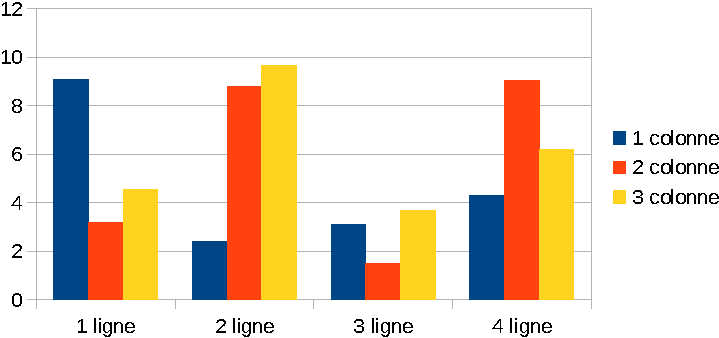
\includegraphics[width=0.7\linewidth]{chart}
	\caption[Diagramme machin]{Diagramme machin. Source : tiré de Tartempion 2010, p. 42 / tiré de ce-site.ch, ref. URL01 / réalisé par Nom Prénom.}
	\label{fig:chart1}
\end{figure}


\subsection{Titre de niveau 3}

Votre texte, votre texte, votre texte, votre texte, votre texte, votre texte, votre texte, votre texte, votre texte, votre texte, votre texte, votre texte, votre texte, votre texte, votre texte, votre texte, votre texte, votre texte Votre texte, votre texte, votre texte, votre texte, votre texte, votre texte, votre texte, votre texte, votre texte, votre texte, votre texte, votre texte, votre texte, votre texte, votre texte, votre texte, votre texte, votre texte Votre texte, votre texte, votre texte, votre texte, votre texte, votre texte, votre texte, votre texte, votre texte, votre texte, votre texte, votre texte, votre texte, votre texte, votre texte, votre texte, votre texte, votre texte.

\begin{table}[tbph!]
	\centering{
		\begin{tabular}{ |l|c|c|c| }
			\hline
			& \textbf{Condition 1} & \textbf{Condition 2} & \textbf{Condition 3} \\
			\hline
			\textbf{Test 1} & X & O & X \\
			\hline
			\textbf{Test 2} & O & X & X \\
			\hline
			\textbf{Test 3} & O & X & O \\
			\hline 
		\end{tabular}
		\caption[Lot de données n°1]{Lot de données n°1. Source: tiré de Tartempion 2010, p. 42 / tiré de ce-site.ch, ref. URL02 / réalisé par Nom Prénom.}
		\label{tab:tableau1}
	}
\end{table}


\subsection{Titre de niveau 3}

Votre texte, votre texte, votre texte, votre texte, votre texte, votre texte, votre texte, votre texte, votre texte, votre texte, votre texte, votre texte, votre texte, votre texte, votre texte, votre texte, votre texte, votre texte.

Votre texte, votre texte, votre texte, votre\footnote{Autre note de bas de page.} texte, votre texte, votre texte, votre texte, votre texte, votre texte, votre texte, votre texte, votre texte, votre texte, votre texte, votre texte, votre texte, votre texte, votre texte.

\begin{figure}[tbph!]
	\centering
	
\includegraphics[width=0.7\linewidth]{diagram}
	\caption[Schéma bidule.]{Schéma bidule. Source : tiré de Tartempion 2010, p. 42 / tiré de ce-site.ch, ref. URL03 / réalisé par Nom Prénom.}
	\label{fig:diagram}
\end{figure}


\section{Titre de niveau 2}

Votre texte, votre texte, votre texte, votre texte, votre texte, votre texte, votre texte, votre texte, votre texte, votre texte, votre texte, votre texte, votre texte, votre texte, votre texte, votre texte, votre texte, votre texte.

\begin{figure}[tbph!]
	\centering
	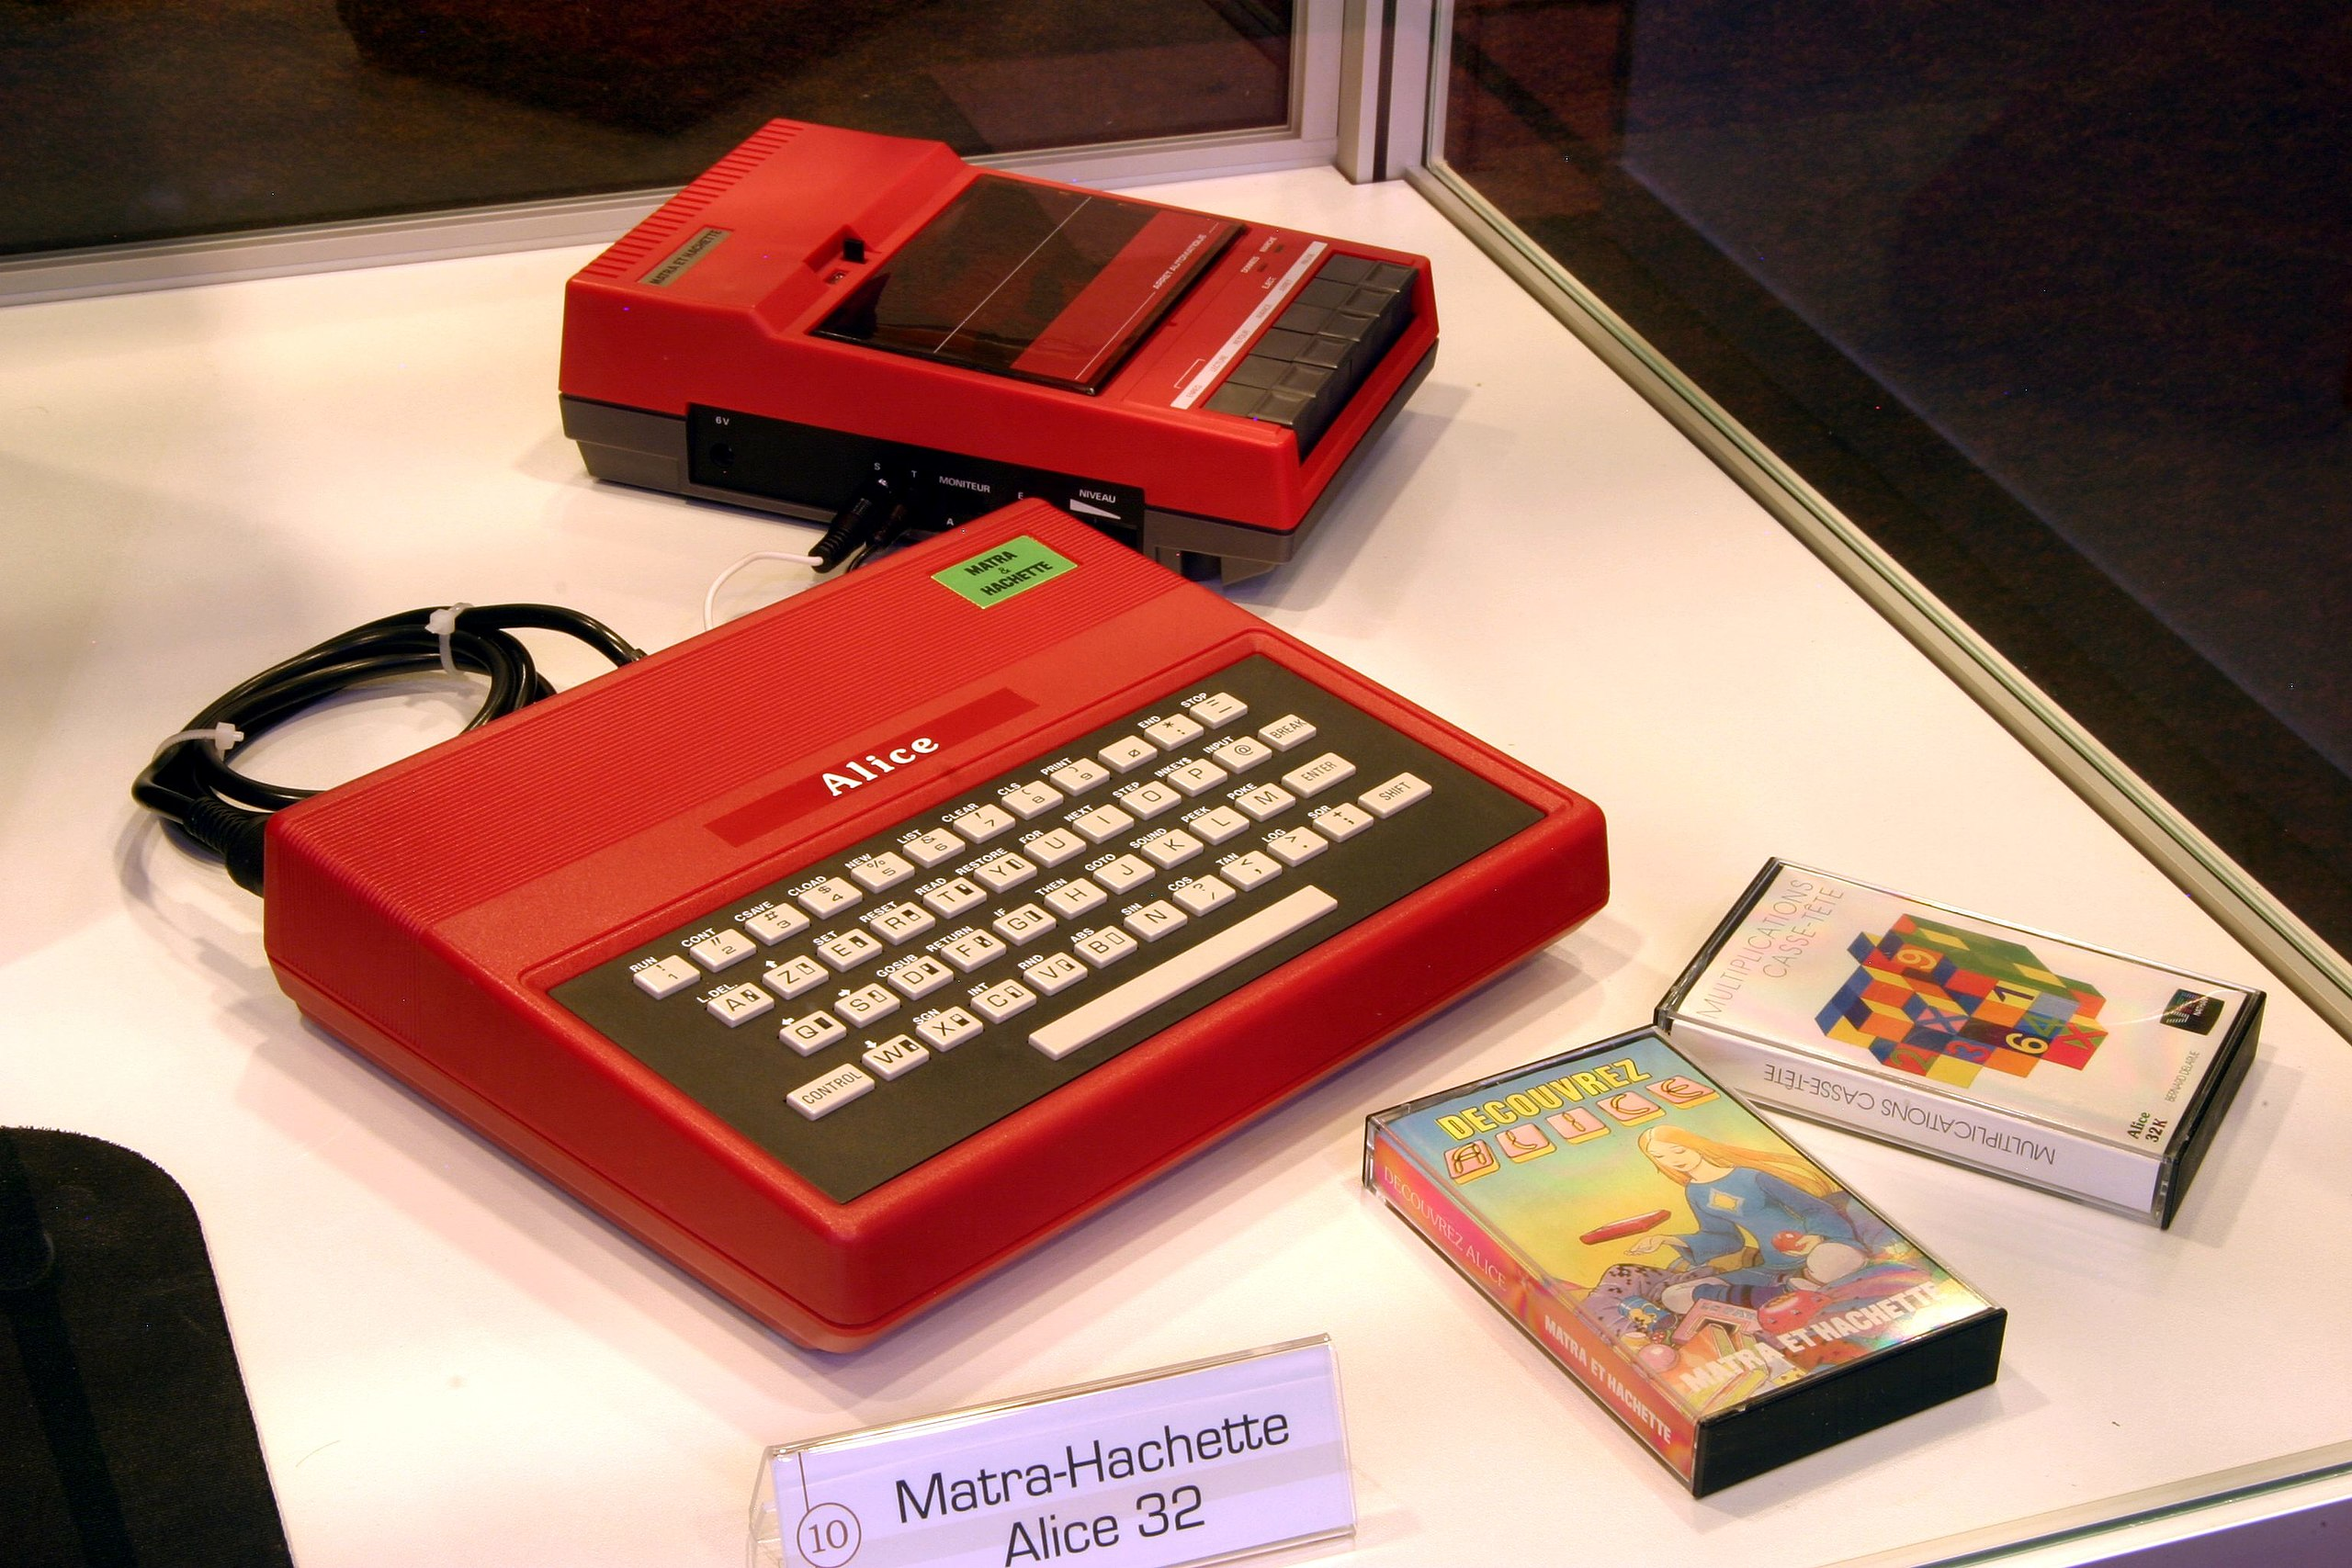
\includegraphics[width=0.7\linewidth]{ordi}
	\caption[Alice, Micro-ordinateur MATRA.]{Alice, Micro-ordinateur MATRA. Source : tiré de Tartempion 2010, p. 42 / tiré de ce-site.ch, ref. URL03 / réalisé par Nom Prénom.}
	\label{fig:image}
\end{figure}


\subsection{Titre de niveau 3}

Votre texte, votre texte, votre texte, votre texte, votre texte, votre texte, votre texte, votre texte, votre texte, votre texte, votre texte, votre texte, votre texte, votre texte, votre texte, votre texte, votre texte, votre texte.


\subsection{Titre de niveau 3}

Votre texte, votre texte, votre texte, votre texte, votre texte, votre texte, votre texte, votre texte, votre texte, votre texte, votre texte, votre texte, votre texte, votre texte, votre texte, votre texte, votre texte, votre texte.

\begin{table}[tbph!]
	\centering{
		\begin{tabular}{ |l|c|c|c| }
			\hline
			& \textbf{Condition 1} & \textbf{Condition 2} & \textbf{Condition 3} \\
			\hline
			\textbf{Test 1} & X & O & X \\
			\hline
			\textbf{Test 2} & O & X & X \\
			\hline
			\textbf{Test 3} & O & X & O \\
			\hline 
		\end{tabular}
		\caption[Lot de données n°2.]{Lot de données n°2. Source: tiré de Tartempion 2010, p. 42 / tiré de ce-site.ch, ref. URL05 / réalisé par Nom Prénom.}
		\label{tab:tableau2}
	}
\end{table}

Votre texte, votre texte, votre texte, votre texte, votre texte, votre texte, votre texte, votre texte, votre texte, votre texte, votre texte, votre texte, votre texte, votre texte, votre texte, votre texte, votre texte, votre texte.


\subsection{Titre de niveau 3}

Votre texte, votre texte, votre texte, votre texte, votre texte, votre texte, votre texte, votre texte, votre texte, votre texte, votre texte, votre texte, votre texte, votre texte, votre texte, votre texte, votre texte, votre texte.

Votre texte, votre texte, votre texte, votre texte, votre texte, votre texte, votre texte, votre texte, votre texte, votre texte, votre texte, votre texte, votre texte, votre texte, votre texte, votre texte, votre texte, votre texte.


\subsection{Titre de niveau 3}

Votre texte, votre texte, votre texte, votre texte, votre texte, votre texte, votre texte, votre texte, votre texte, votre texte, votre texte, votre texte, votre texte, votre texte, votre texte, votre texte, votre texte, votre texte.

Votre texte, votre texte, votre texte, votre texte, votre texte, votre texte, votre texte, votre texte, votre texte, votre texte, votre texte, votre texte, votre texte, votre texte, votre texte, votre texte, votre texte, votre texte.